\section{Results - Elicitation of parameters}
\label{ResultsElicitation}
%I må gerne tjekke oversættelsen på SQ og labels, så sletter vi de danske SQ efterfølgende og skriver det vigtige
%
Based on the 10 categories, variables were elicited according to the criterion of a) being an influencing variable and b) the possibility of formulating the variable as a scale question. The field study was conducted on Danish speaking test subjects, and the variables are therefore listed in both English and Danish. The scale questions are all presented on a \textit{Visual Analoge Scale} (VAS) with closed anchor points and are either bi- or unipolar. If the scale is bipolar a midpoint will be marked either with or without a label. A bipolar scale without a label will be noted with \textit{No label}, whereas an unipolar scale which does not contain a midpoint will be noted with a \textit{-}. 

In the following the 23 derived scales (noted \textit{S}), along with the specific scale question (SQ), will be presented in corresponding order as presented for the test subjects in Experiment 2 and sorted by each page ind the robots interface. An example of each set of scales is given, to illustrate how they were presented in the experiment.\\ 
\subsection{Page 1}
\noindent
SQ1: How do think the screen on the robot reacted? \\%(Hvordan synes du, at skærmen på robotten reagerede?)\\
SQ2: How did you experience the robot? \\ %(Hvordan oplevede du robotten?)\\
SQ3: How was it to use the robot?\\% (Hvordan var det at bruge robotten?)\\
SQ4: How did you experience the robot's movements? \\%(Hvordan oplevede du robottens bevægelser?)\\%
\begin{table}[H]
	\centering
\caption{Scale labels PAGE 1}
	\label{tab:ScalesPage1} 
	\begin{tabular}{l|c|c|c}
		S     & Left label & Mid point & Right label \\\hline
		1   & \makecell{Extremely bad\\(Ekstremt dårligt)}  & No label & \makecell{Extremely well \\(Ekstremt godt)}        \\\hline
		2   & \makecell{Extremely unwelcoming \\(Ekstremt afvisende)} & No label & \makecell{Extremely welcoming \\(Ekstremt imødekommende)}         \\\hline
		3   & \makecell{Extremely difficult \\(Ekstremt svært)} & No label & \makecell{Extremely easy \\(Ekstremt nemt)}         \\\hline
	 	4   & \makecell{Extremely wild \\(Ekstremt vilde)} & No label & \makecell{Extremely calm \\(Ekstremt rolige)}               
	\end{tabular}        
\end{table}
\noindent
%
\begin{figure}[H]
\centering

\includegraphics[width = 0.49\textwidth]{Figure/TilpassetSkaermensReaktion}
\setlength\abovecaptionskip{-1.2\baselineskip} 
\caption{Example of a bipolar scale relevant for the scale question: \textit{How do think the screen on the robot reacted?}, rated from \textit{Extremely bad} to \textit{Extremely well}.}
\label{fig:TilpassetSkaermensReaktion}
\end{figure}
\noindent
% 
\subsection{Page 2}
\noindent
SQ5: I think that the robot stopped... \\%(Jeg synes, at robotten stoppede...)\\
SQ6: I think that the robot's speed is... \\%(Jeg synes, at robottens hastighed er...)\\ 
SQ7: I think that the robot's height is... \\%(Jeg synes, at robottens højde er..)\\
%
\begin{table}[H]
	\centering
\caption{Scale labels PAGE 2}
	\label{tab:ScalesPage2} 
	\begin{tabular}{l|c|c|c}
		S     & Left label & Mid point & Right label \\\hline
		5   & \makecell{Way too close\\(Alt for tæt på)}  & No label & \makecell{Way too far \\(Alt for langt fra)}        \\\hline
		6   & \makecell{Way too slow\\(Alt for langsom)} & \makecell{Fine\\(Fin)} & \makecell{Way too fast \\(Alt for hurtig)}         \\\hline
		7   & \makecell{Way too low \\(Alt for lav)} & \makecell{Fine\\(Fin)} & \makecell{Way too high\\(Alt for høj)}                
	\end{tabular}        
\end{table}
\noindent
%
\begin{figure}[H]
\centering
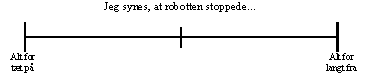
\includegraphics[width = 0.49\textwidth]{Figure/TilpassetRStoppede}
\setlength\abovecaptionskip{-1.2\baselineskip} 
\caption{Example of a bipolar scale relevant for the scale question: \textit{I think that the robot stopped...}, rated from \textit{Way too close} to \textit{Way too far}.}
\label{fig:TilpassetRStoppede}
\end{figure}
\noindent
% 
\subsection{Page 3 and 4}
\noindent
SQ8: I feel that the robot can help me\\% (Jeg føler, at robotten kan hjælpe mig)\\
SQ9: I think that the robot was obstructing me\\%(Jeg synes, at robotten stod i vejen)\\
SQ10: I feel safe around the robot\\%(Jeg føler mig tryg ved robotten)\\
SQ11: The robot startled me\\ %(Robotten gjorde mig forskrækket)\\
SQ12: I like to be served by the robot\\% (Jeg kan godt lide at blive betjent af robotten)\\
SQ13: I counted on the robot to lead me to the location I chose\\% (Jeg regnede med, at robotten fulgte mig hen til det sted jeg valgte)\\
%
\begin{table}[H]
	\centering
\caption{Scale labels PAGE 3 and 4}
	\label{tab:ScalesPage3} 
	\begin{tabular}{l|c|c|c}
		S     & Left label & Mid point & Right label \\\hline
		8-13   & \makecell{Completely disagree\\(Helt uenig)}  & No label & \makecell{Completely agree\\(Helt enig)}                      
	\end{tabular}        
\end{table}
\noindent
%
\begin{figure}[H]
\centering
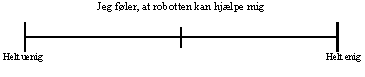
\includegraphics[width = 0.49\textwidth]{Figure/TilpassetRobottenKanHjaelpe}
\setlength\abovecaptionskip{-1.9\baselineskip} 
\caption{Example of a bipolar scale relevant for the scale question: \textit{I feel that the robot can help me}, rated from \textit{Completely disagree} to \textit{Completely agree}.}
\label{fig:TilpassetRobottenKanHjaelpe}
\end{figure}
\noindent
% 
\subsection{Page 5}
\noindent
SQ14: How personal did you experience the robot's help?\\% (Hvor personlig oplevede du robottens hjælp?)\\
SQ15: How surprised were you by the robot's approach?\\% (Hvor overrasket blev du over robottens henvendelse?)\\
For each of the two scale questions the chosen labels are listed in \autoref{tab:ScalesPage5}. 
%
\begin{table}[H]
	\centering
\caption{Scale labels PAGE 5}
	\label{tab:ScalesPage5} 
	\begin{tabular}{l|c|c|c}
		S     & Left label & Mid point & Right label \\\hline
		14   & \makecell{Not at all personal\\(Slet ikke personlig)}  & - & \makecell{Extremely personal\\(Ekstremt personlig)}        \\\hline
		15   & \makecell{Not at all surprised\\(Slet ikke overrasket)} & - & \makecell{Extremely surprised \\(Ekstremt overrasket)}               
	\end{tabular}        
\end{table}
\noindent
%
\begin{figure}[H]
\centering
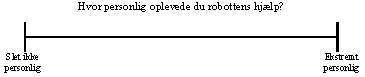
\includegraphics[width = 0.49\textwidth]{Figure/TilpassetPersonligHjaelp}
\setlength\abovecaptionskip{-1.2\baselineskip} 
\caption{Example of an unipolar scale relevant for the scale question: \textit{How personal did you experience the robots help?}, rated from \textit{Not at all personal} to \textit{Extremely personal}.}
\label{fig:TilpassetPersonligHjaelp}
\end{figure}
\noindent
% 
\subsection{Page 6}
\noindent
SQ16: What do you think about the robot?\\% (Hvad synes du om robotten)\\
This scale question covers scales 16-19. 
%
\begin{table}[H]
	\centering
\caption{Scale labels PAGE 6}
	\label{tab:ScalesPage6} 
	\begin{tabular}{l|c|c|c}
		S     & Left label & Mid point & Right label \\\hline
		16   & \makecell{Not at all annoying\\(Slet ikke irriterende)}  & - & \makecell{Extremely annoying \\(Ekstremt irriterende)}        \\\hline
		17   & \makecell{Not at all elegant \\(Slet ikke elegant)} & - & \makecell{Extremely elegant \\(Ekstremt elegant)}         \\\hline
		18   & \makecell{Not at all exciting\\(Slet ikke spændende)} & - & \makecell{Extremely exciting \\(Ekstremt spændende)}         \\\hline
	 	19   & \makecell{Not at all cute\\(Slet ikke sød)} & - & \makecell{Extremely cute \\(Ekstremt sød)}               
	\end{tabular}        
\end{table}
\noindent
%
\subsection{Page 7}
\noindent
SQ17: What else do you think about the robot?\\%(Hvad synes du ellers om robotten?)\\
This scale question covers scales 20-23. 
%
\begin{table}[H]
	\centering
\caption{Scale labels PAGE 7}
	\label{tab:ScalesPage7} 
	\begin{tabular}{l|c|c|c}
		S    & Left label & Mid point & Right label \\\hline
		20   & \makecell{Not at all cool\\(Slet ikke sej)}  & - & \makecell{Extremely cool \\(Ekstremt sej)}        \\\hline
		21   & \makecell{Not at all intrusive \\(Slet ikke anmassende)} & - & \makecell{Extremely intrusive \\(Ekstremt anmassende)}         \\\hline
		22   & \makecell{Not at all funny\\(Slet ikke sjov)} & - & \makecell{Extremely funny \\(Ekstremt fun)}         \\\hline
	 	23   & \makecell{Not at all human \\(Slet ikke menneskelig)} & - & \makecell{Extremely human \\(Ekstremt menneskelig)}               
	\end{tabular}        
\end{table}
\noindent
%
Based on the affinity diagram a 24th parameter was derived, this parameter will not be presented along side the aforementioned scales but will be included in a separate demographic page as it does not directly concern the robot. The parameter is formulated in the scale question: \textit{How fond of technology are you?}, which will be evaluated on an unipolar scale, similar to the other unipolar scales, with anchor points: \textit{Not at all fond} (slet ikke glad) and \textit{Extremely fond} (ekstremt glad).\\  

\noindent
When comparing the variables for HRI found in this study with variables for HRI from previous conducted studies on social robots \cite{PDF:ExploringInfluencingVariable}, \cite{PDF:SharingALifeHarvey}, \cite{PDF:InTheCompanyofRobots}, \cite{PDF:CloseButNotStuck}, \cite{PDF:TheImpactOfTraveler}, \cite{PDF:HumanRobotEmodiedInteraction}, \cite{PDF:RecommendationEffects}, variables such as distance, anthropomorphism, height, speed, movement, trust, enjoyment, technological knowledge, and usefulness reoccur. New variables were found compared with previous mentioned studies these are: Elegance, cute, cool, startled, exciting, welcoming, obstructive, robot help as personal, and wether the encounter with the robot was surprising. However, these might be measured indirectly in the aforementioned studies.

Accordring to \cite{PDF:HowSocialDistanceShapesHRI} \textit{social distance} has an effect on HRI. Even though the subjects in AAL did not mention it specifically it seems that this is due to \textit{power distance}, where the subjects feel in control as they were the dominant part and the robot was the subordinate in the interaction. Furthermore this could also be due to the given HRI task was cooperative as the robot's purpose was to help the subject to a specific location of their choosing. When focusing on \textit{task distance} when in cooperative tasks it seems as if the subjects acted more friendly, intimate, and involved in the interaction with the robot, which is based on all the positive comments from subjects \fxnote{Jeg forstår ikke denne sætning. Måske en omskrivning? - Korn.}
 
  




